\documentclass{beamer}

\usetheme{Antibes}

\title{The Bitcoin Mining Protocol}

\author[Lamur, Duran]{Jules Lamur\inst{1} \and Jeremy Duran\inst{1}}
\institute
{
    \inst{1}
    Université de Toulouse 3 --- Paul Sabatier
}
\date[2019]{English Course Oral Presentation 2019}

\subject{Computer Science}

\AtBeginSection[]
{
    \begin{frame}
        \frametitle{Table of Contents}
        \tableofcontents[
            currentsection,
            hideothersubsections]
    \end{frame}
}

\begin{document}

\frame{\titlepage}

\begin{frame}
    \frametitle{Table of Contents}
    \tableofcontents[hidesubsections]
\end{frame}

\section{Introduction}

\begin{frame}
    \begin{center}
        
\includegraphics[height=3cm]{bitcoin_logo.png}
    \end{center}

    \textbf{Bitcoin} is a crypto-currency based on decentralized consensus rules.
    \pause

    The \textbf{Bitcoin Protocol} is the specification of said rules.
\end{frame}

\subsection{History}

\begin{frame}
    \begin{itemize}
        \item Created in 2008 by \textbf{Satoshi Nakamoto} (anonymous
            individual or group).

        \item Satoshi released, along with the very first Bitcoin
            implementation, a white paper named \textit{Bitcoin: A Peer-to-Peer
            Electronic Cash System}\footnote{https://bitcoin.org/bitcoin.pdf}
            where he describes the purpose and motivations of the Bitcoin
            creation.

        \item A lot of forks exist, \textit{e.g.} Litecoin, Bitcoin Cash,
            Dogecoin. The ``orignal'' Bitcoin implementation is known as
            \textbf{Bitcoin Core}.

        \item Nowadays, the Bitcoin Core source-code is maintained by a lot of
            different people around the world, and all forks follows more or
            less precisely the rules implemented by the Core.
    \end{itemize}
\end{frame}

\section{The Life of a Transaction}

\begin{frame}
    \begin{center}
        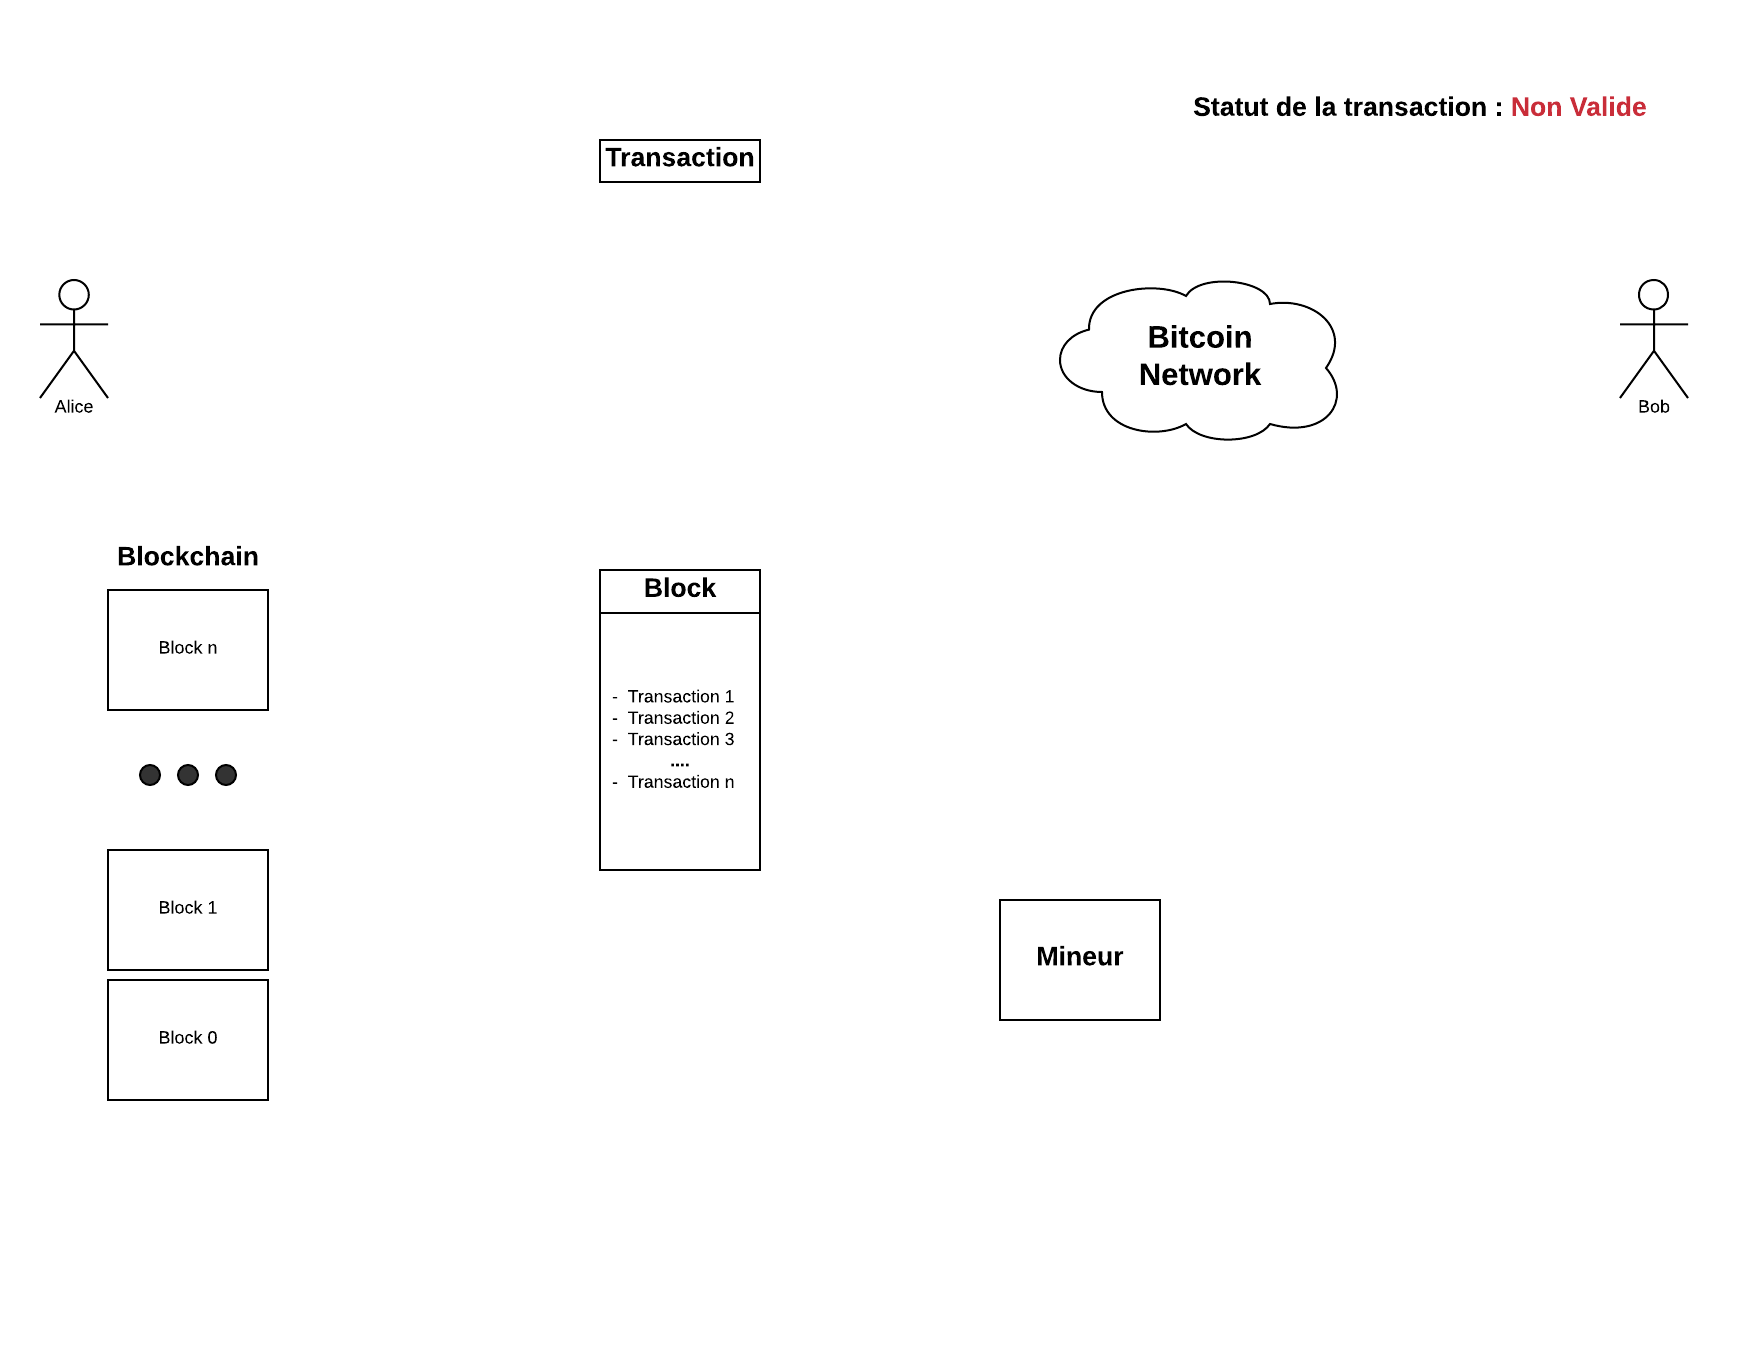
\includegraphics[height=8cm]{images/explanation-0.png}
    \end{center}
\end{frame}

\begin{frame}
    \begin{center}
        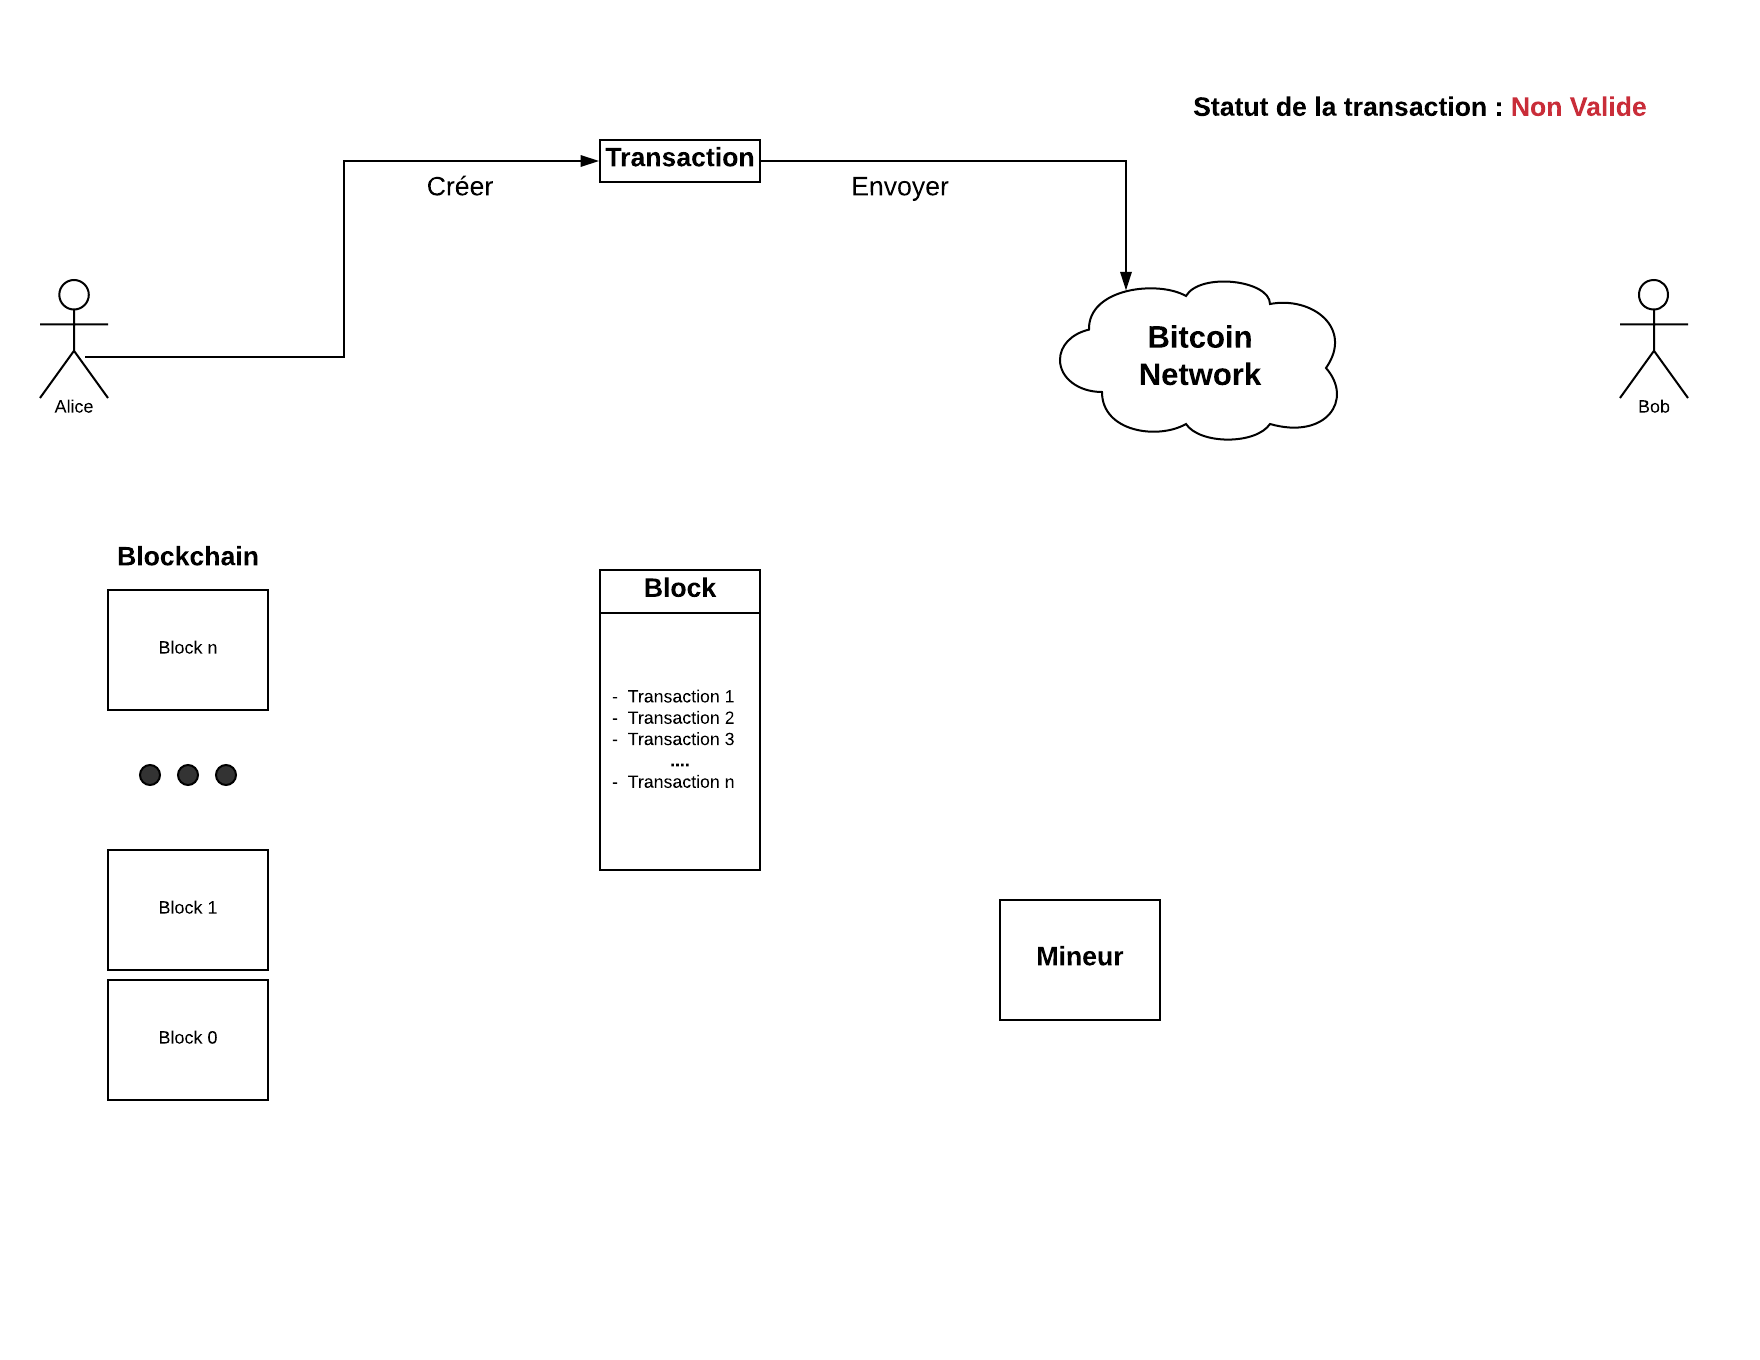
\includegraphics[height=8cm]{images/explanation-2.png}
    \end{center}
\end{frame}

\begin{frame}
    \begin{center}
        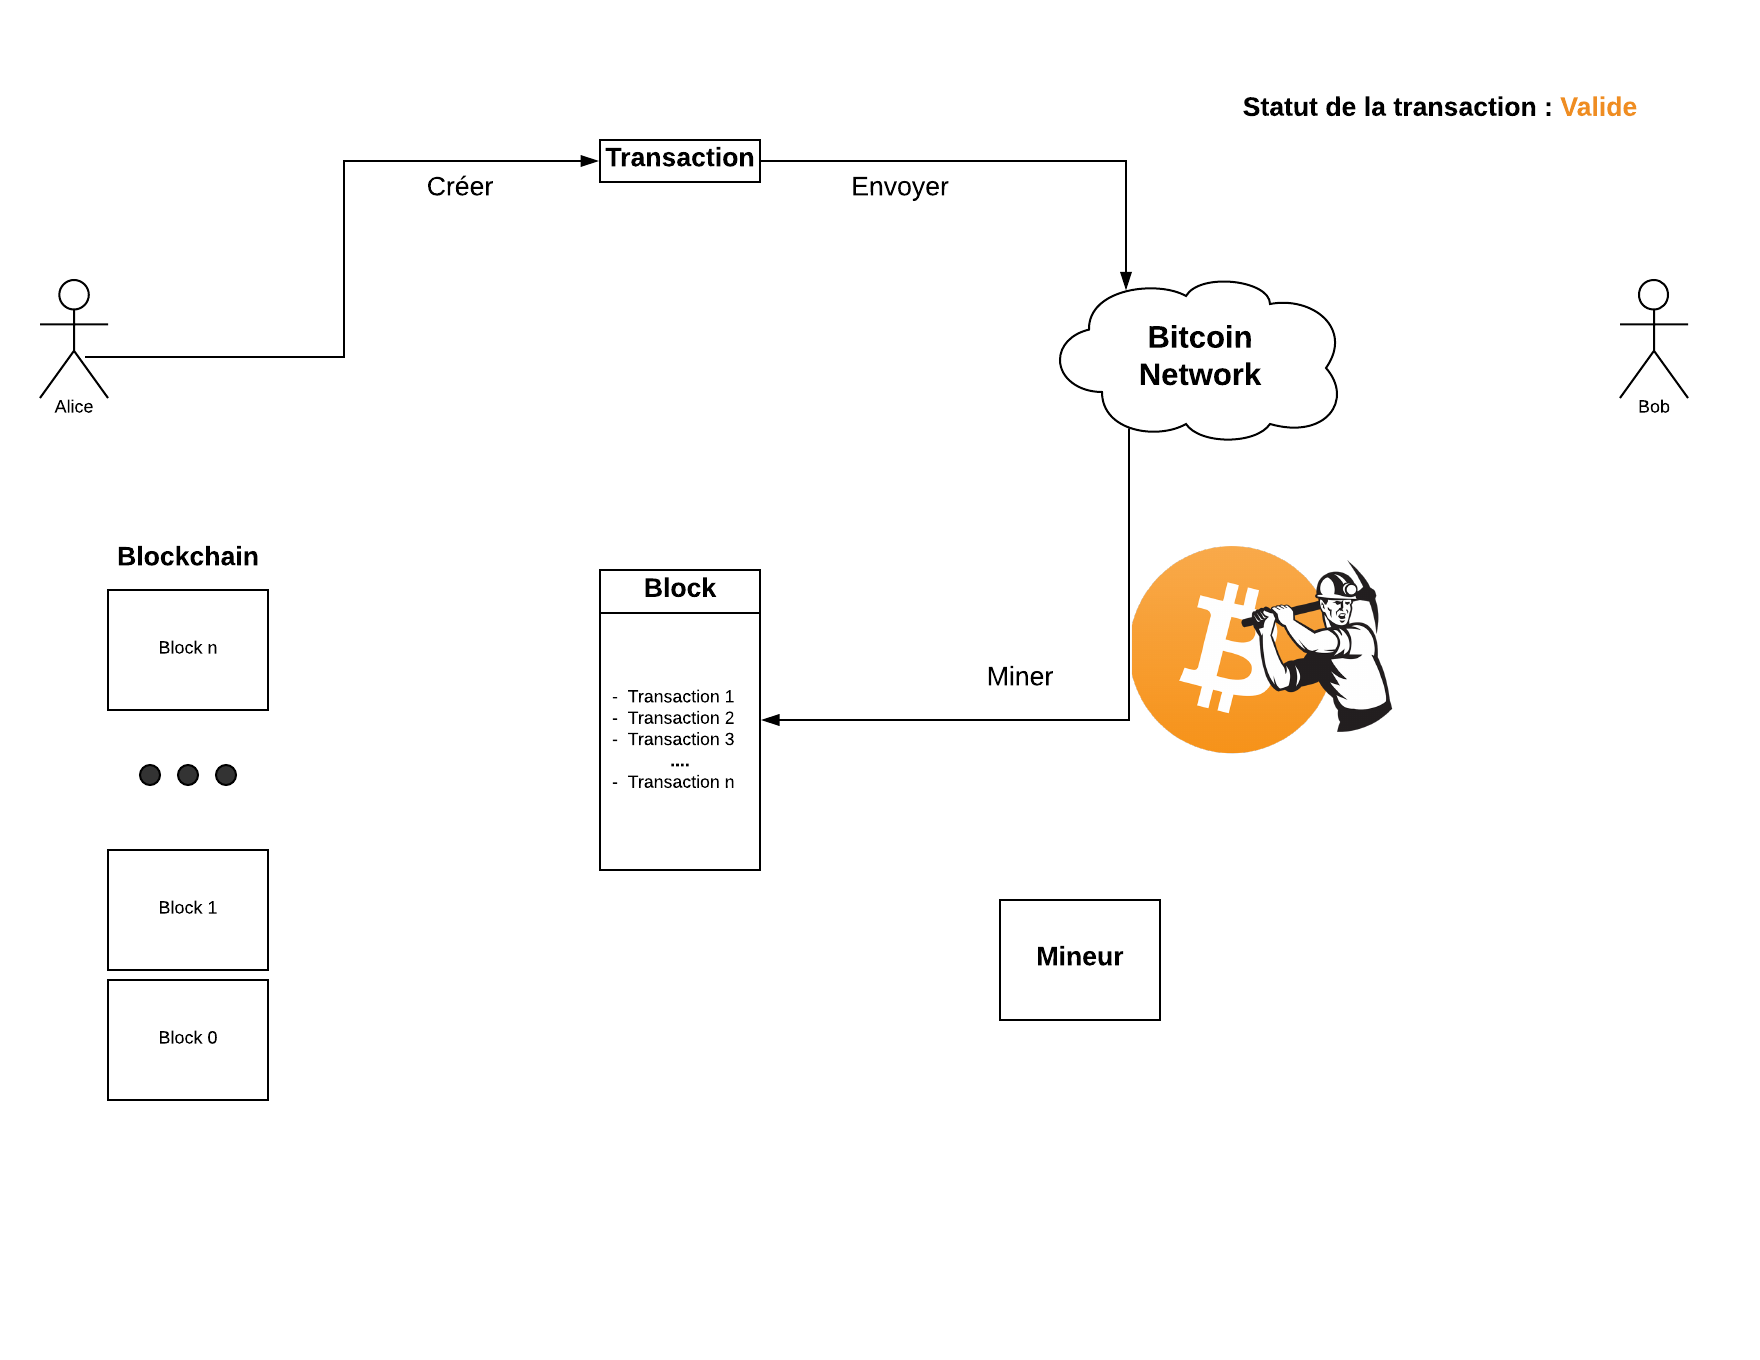
\includegraphics[height=8cm]{images/explanation-3.png}
    \end{center}
\end{frame}

\begin{frame}
    \begin{center}
        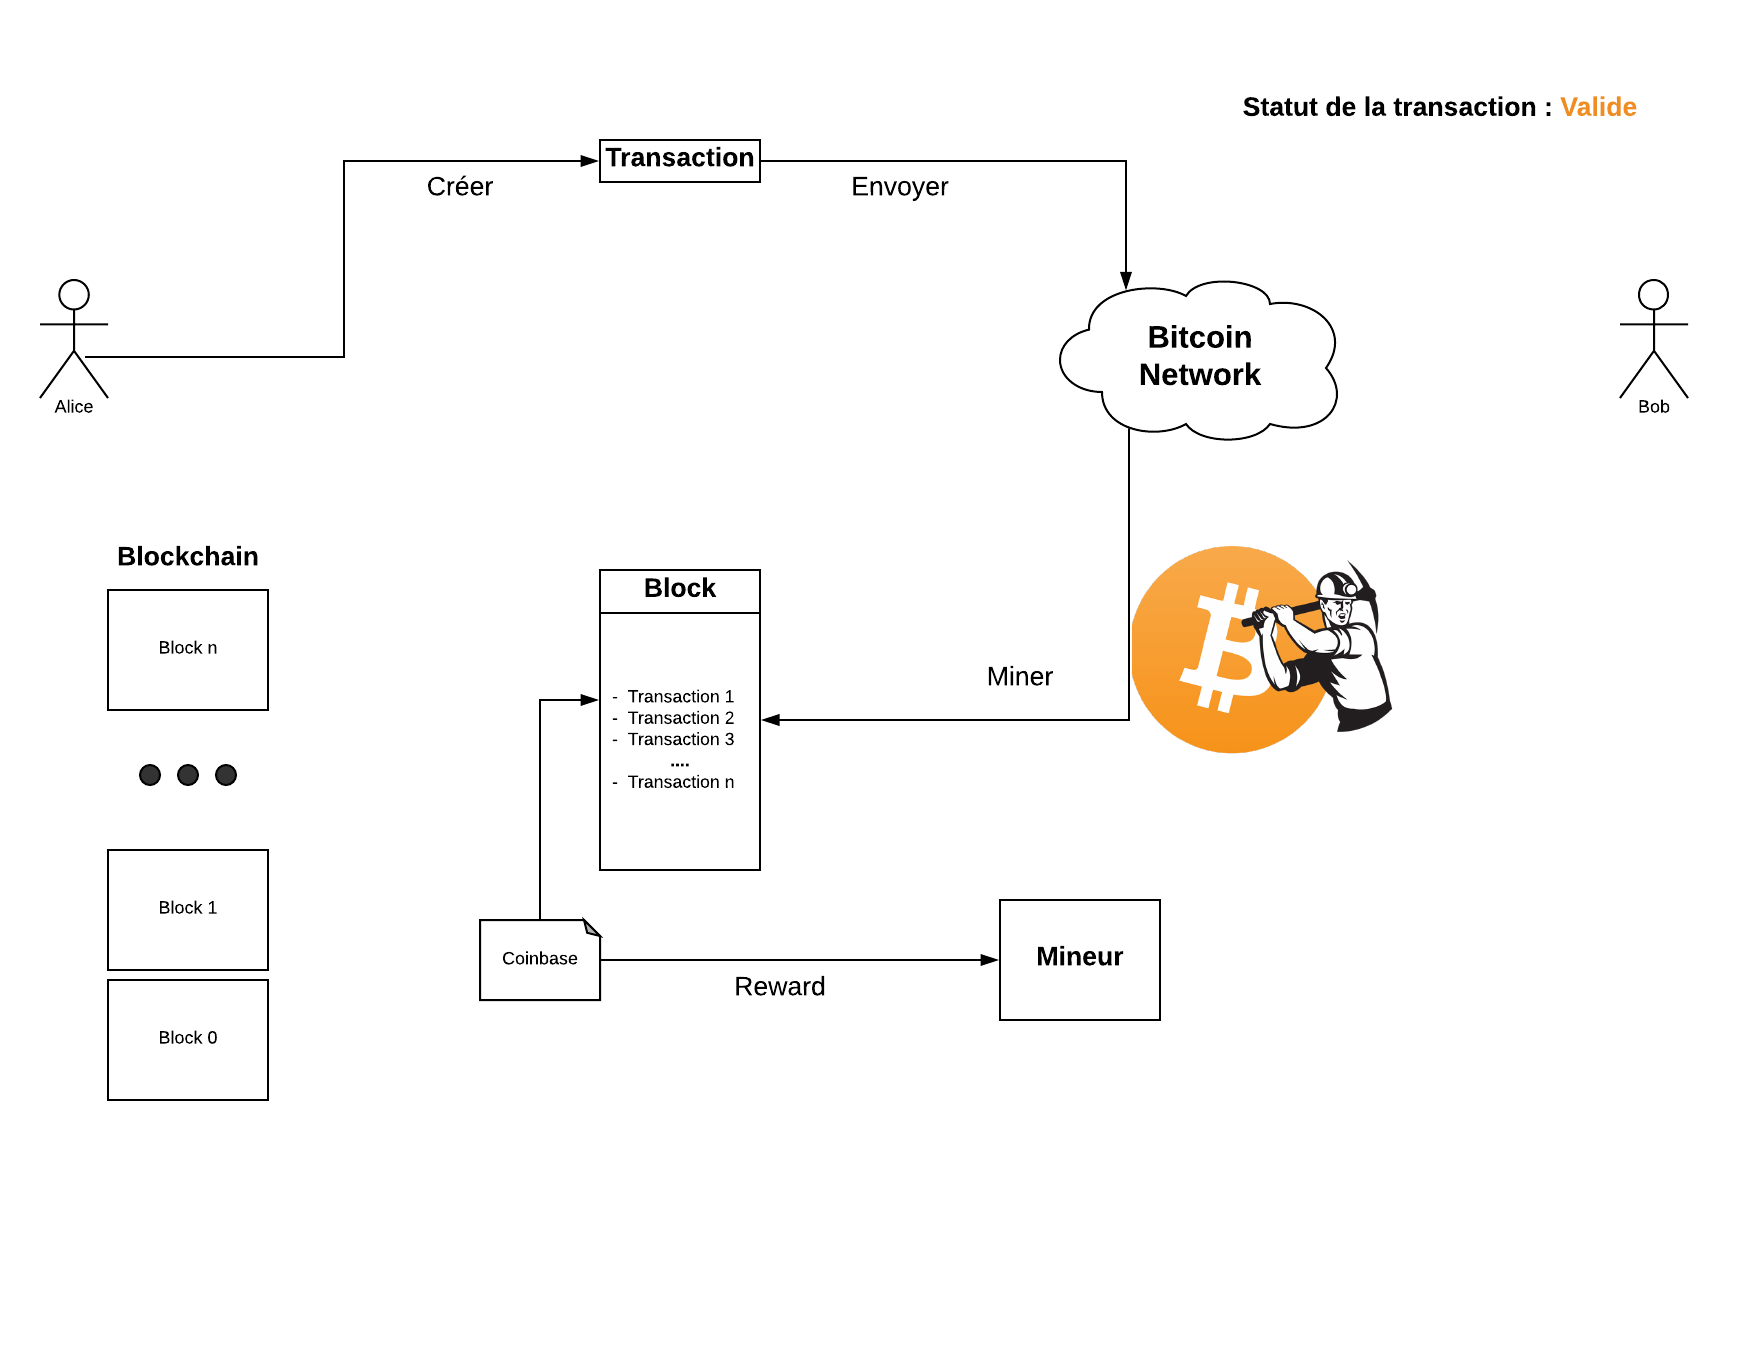
\includegraphics[height=8cm]{images/explanation-4.png}
    \end{center}
\end{frame}

\begin{frame}
    \begin{center}
        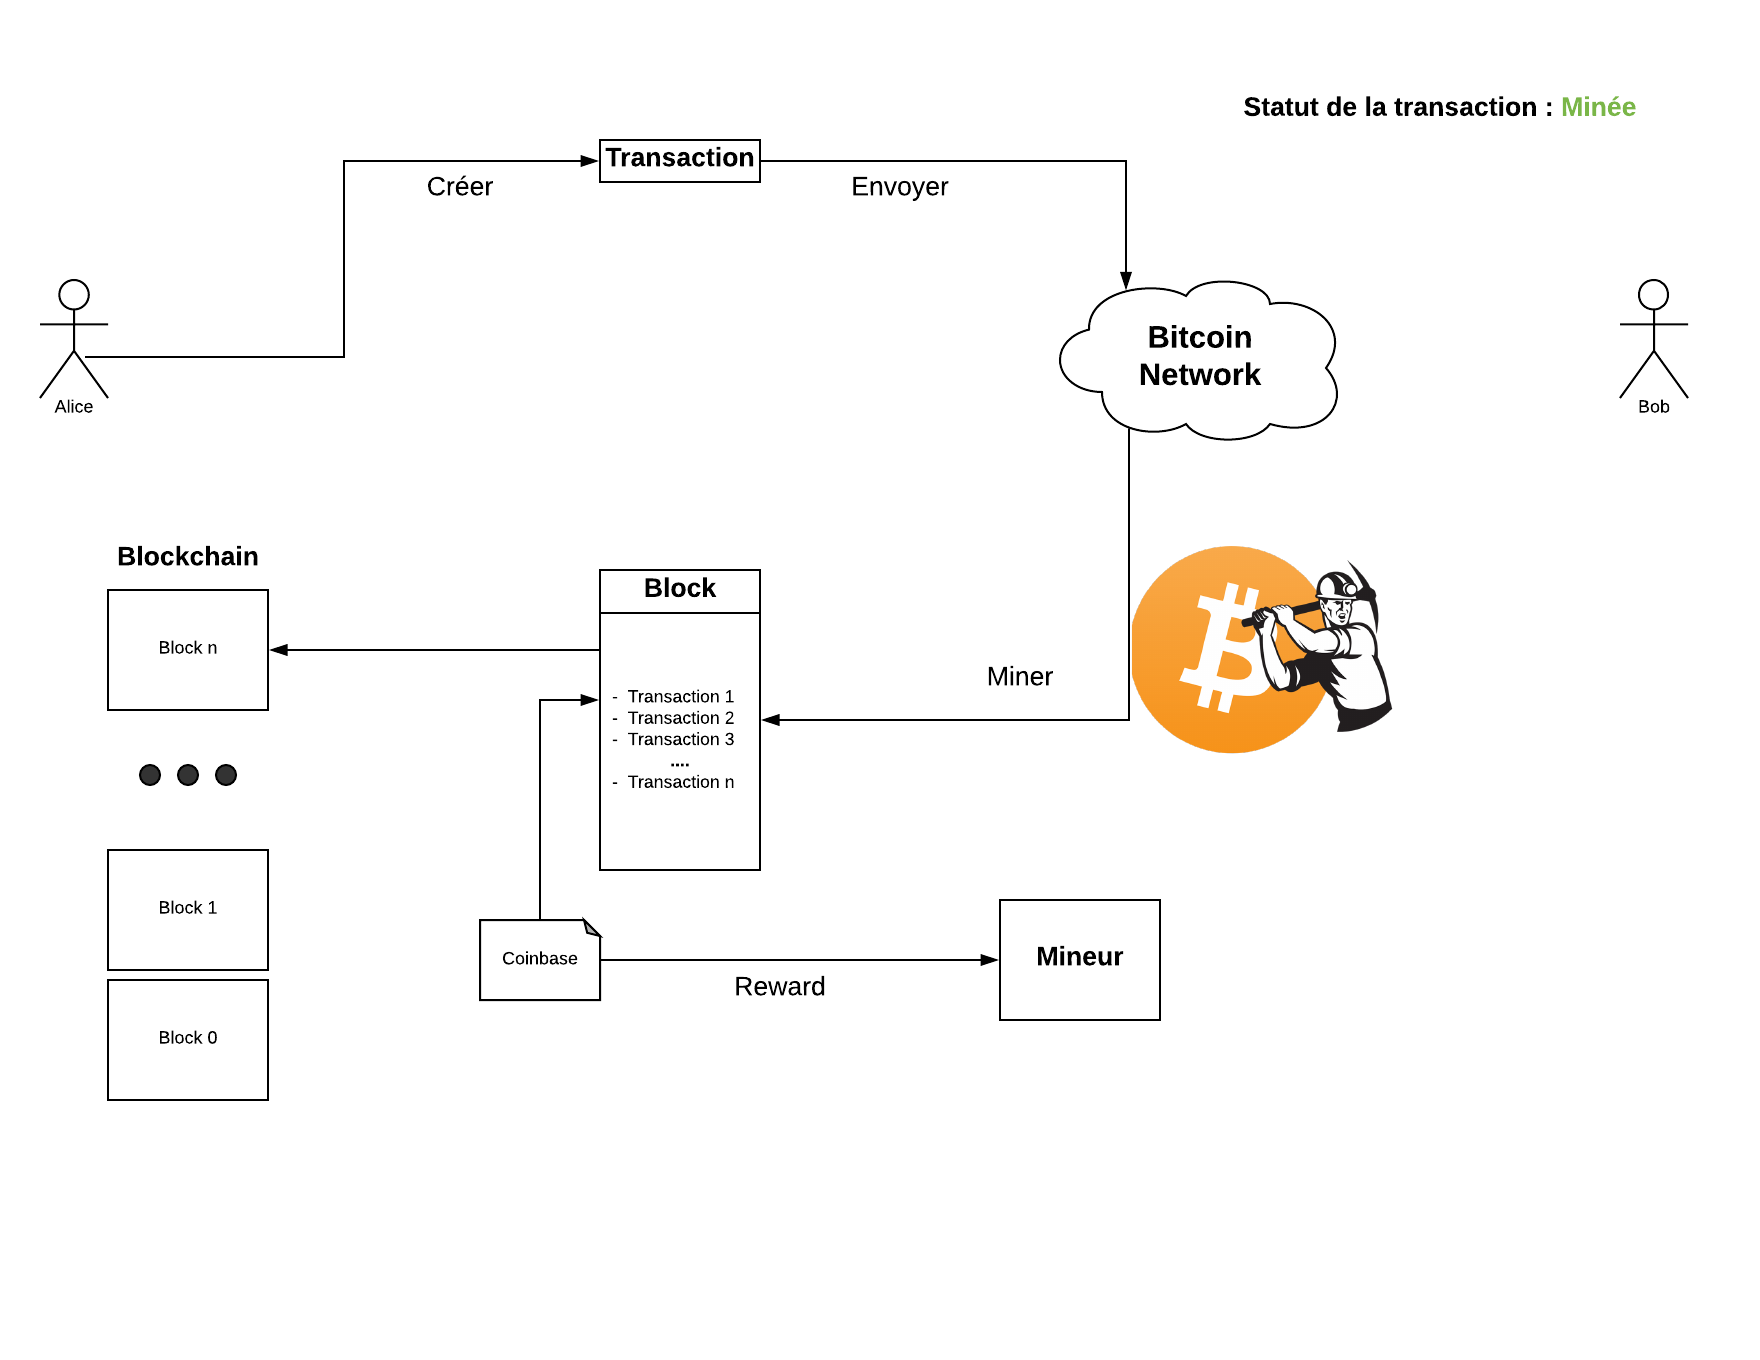
\includegraphics[height=8cm]{images/explanation-5.png}
    \end{center}
\end{frame}

\begin{frame}
    \begin{center}
        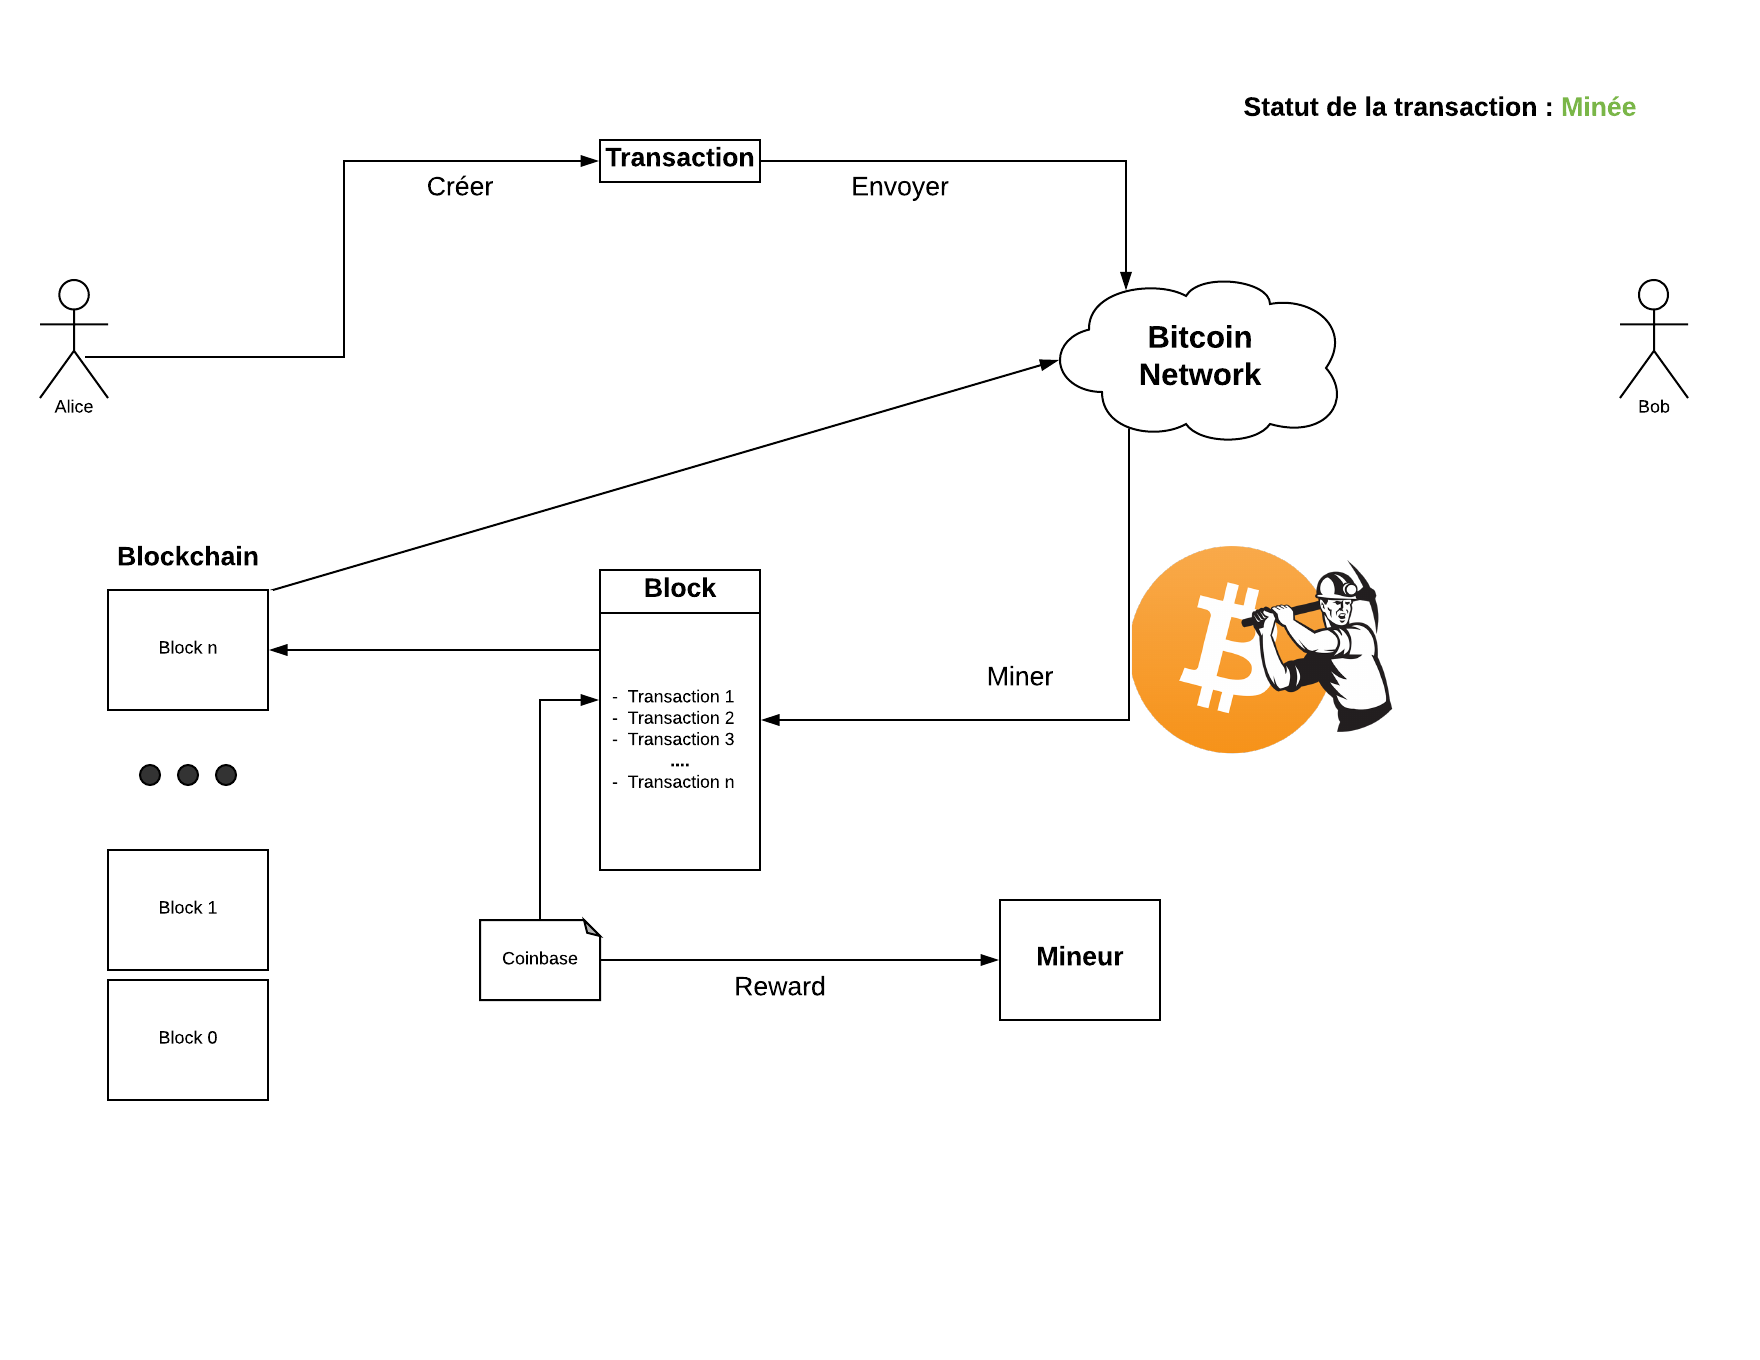
\includegraphics[height=8cm]{images/explanation-6.png}
    \end{center}
\end{frame}

\begin{frame}
    \begin{center}
        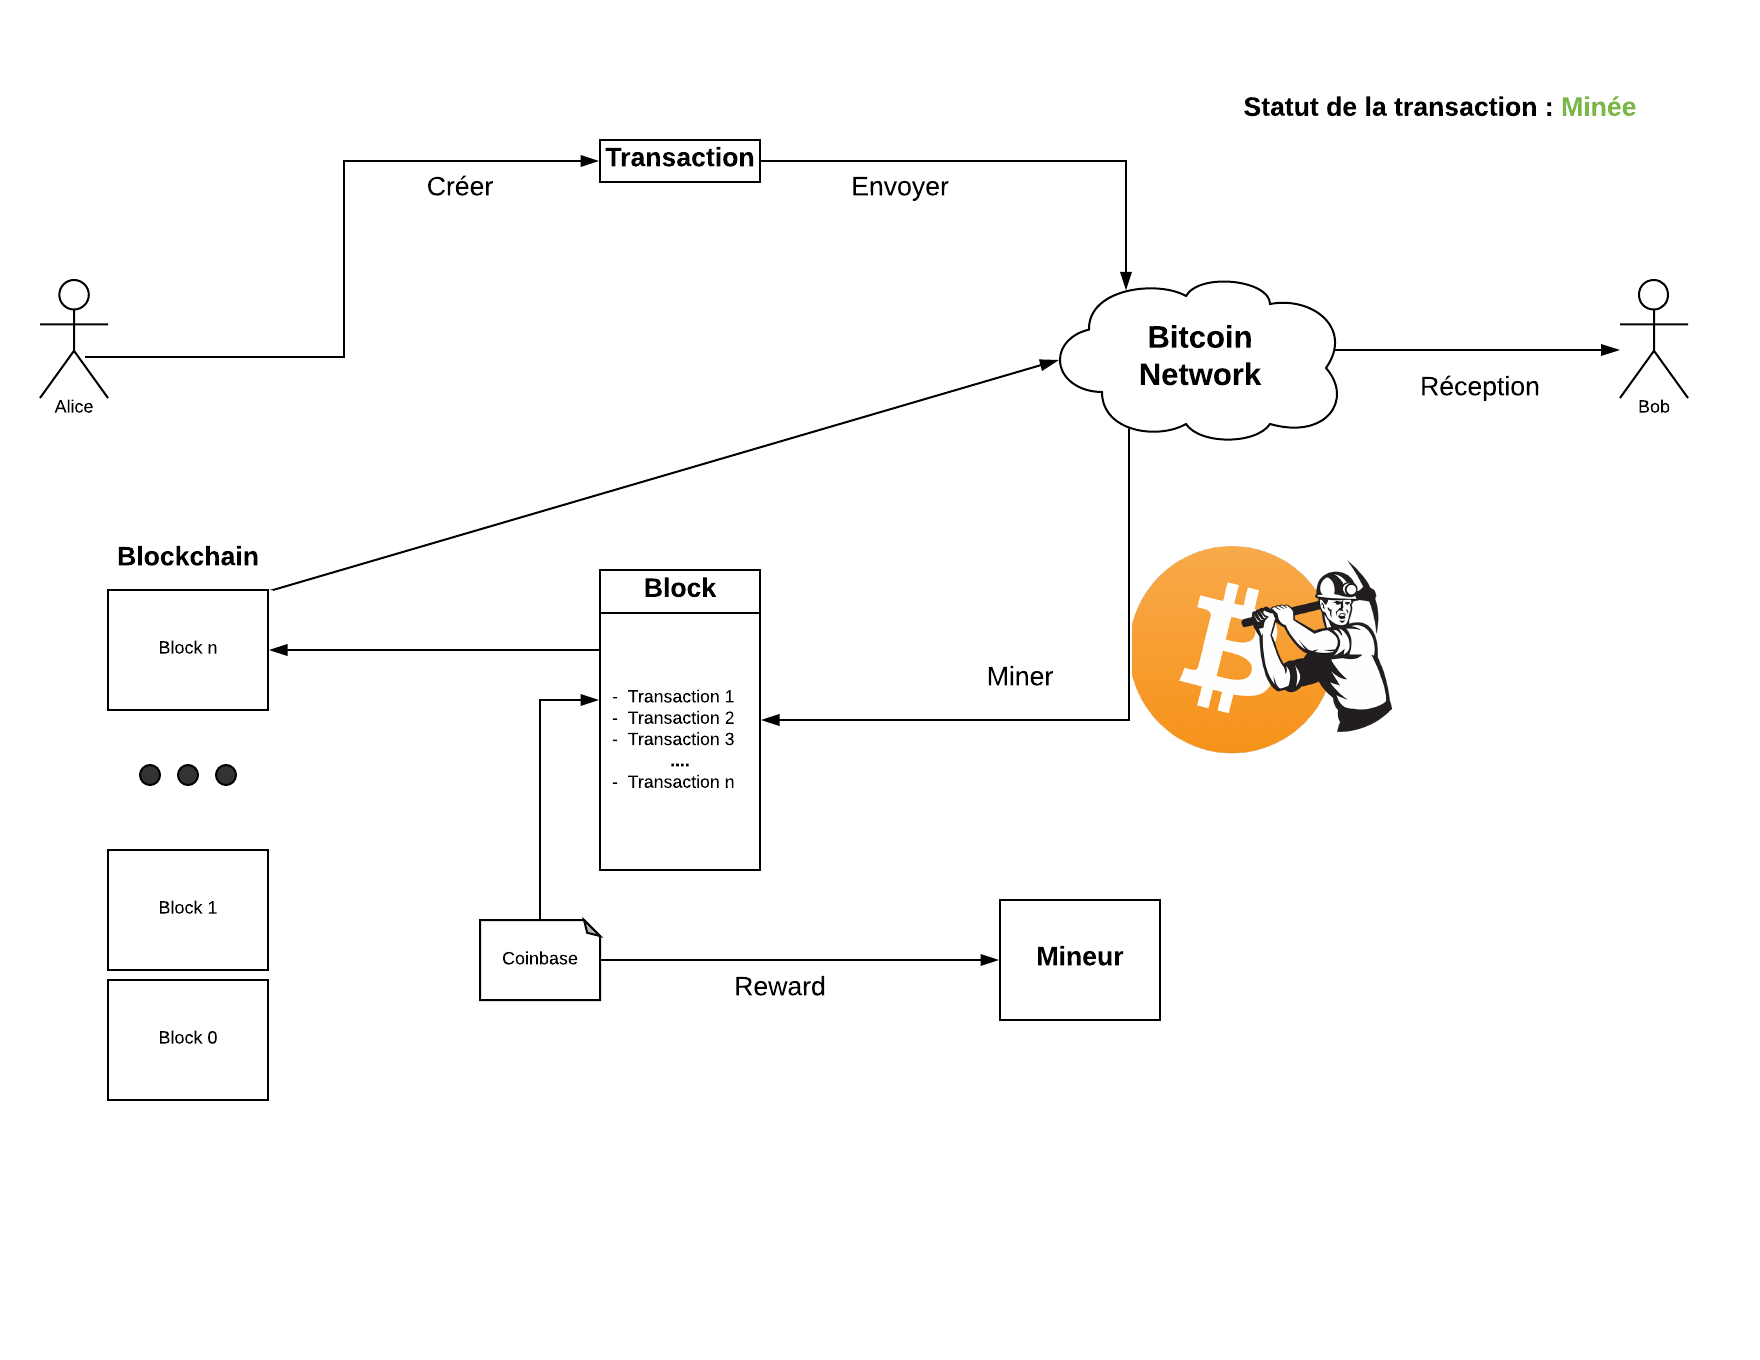
\includegraphics[height=8cm]{images/explanation-7.png}
    \end{center}
\end{frame}

\begin{frame}
    \begin{center}
        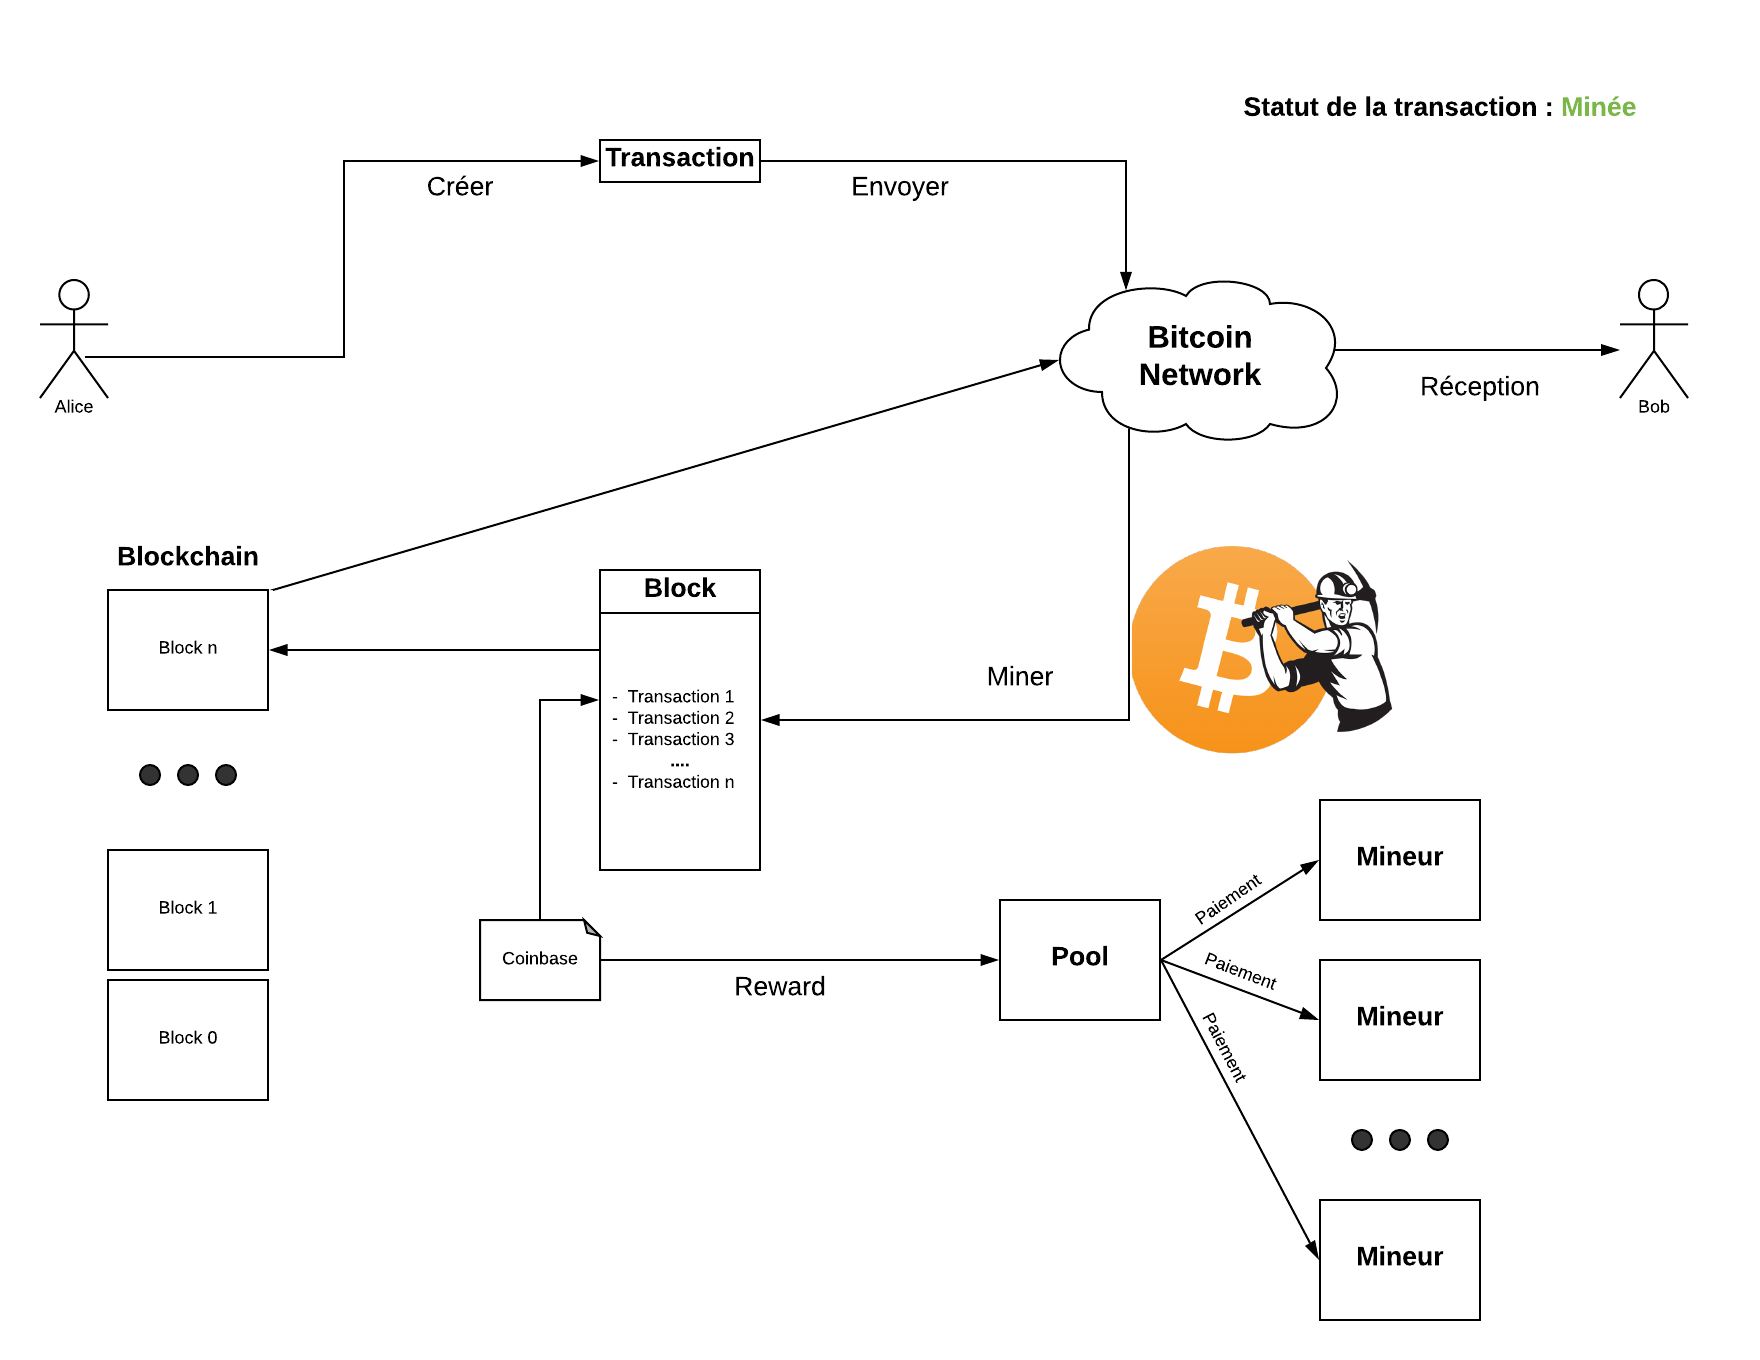
\includegraphics[height=8cm]{images/explanation-8.png}
    \end{center}
\end{frame}

\section{Mining}
\subsection{Prerequisites}

\begin{frame}
    \begin{itemize}
        \item Asymetric cryptography
        \item Hashing functions
    \end{itemize}
\end{frame}

\subsection{Proof of Work}

\begin{frame}
\end{frame}

\end{document}
